% !TeX spellcheck = en_US
\documentclass[
english,
openany,
draft = false,
twoside = true,
fleqn
]{scrbook}
\usepackage{learning-notes}

\author{Huu Duc Nguyen}
\authordegreefront{}
\authordegreeback{ M.Sc.}
\subject{Computer Vision}
\title{Computer Vision Notes}
\date{29 March 2022}

\begin{document}
	\frontmatter
	\TitlePage
	\tableofcontents
	
	\mainmatter
	% !TeX spellcheck = en_GB
\chapter*{Abbreviations}
\addcontentsline{toc}{chapter}{Abbreviations}

\begin{acronym}[LONGEST]
\acro{AI}{Artificial Intelligence}
\acro{AGI}{Artificial General Intelligence}
\acro{ML}{Machine Learning}
\acro{DL}{Deep Learning}
\acro{CS}{Computer Science}
\acro{CV}{Computer Vision}
\acro{RL}{Reinforcement Learning}
\acro{NLP}{Natural Language Processing}
\acro{GPU}{Graphics Processing Unit}
\acro{CPU}{Central Processing Unit}

% Conferences
\acro{ICML}{\href{https://icml.cc/}{International Conference on Machine Learning}}

\acro{prob}[prob.]{probability}
\acro{param}[params.]{parameters}
\acro{algor}[algor.]{algorithms}
\acro{info}[info.]{information}
\acro{aka}[a.k.a.]{also known as}
\acro{wrt}[w.r.t.]{with regard to}
\acro{no}[no.]{number of}
\acro{func}[func.]{function}
\acro{vs}[vs.]{versus}
\acro{freq}[freq.]{frequency}
\acro{st}[s.t.]{subject to}

\acro{iid}[i.i.d.]{independent \& identically distributed}
\acro{LSI}{linear shift invariant}
\acro{pdf}[pdf.]{Probability Density Function}
\acro{MLE}{Maximum Likelihood Estimation}
\acro{MAP}{Maximum A Posteriori}
\acro{MoG}{Mixture of Gaussians}
\acro{SVM}{State Vector Machine}

% Gradient descent
\acro{GD}{Gradient Descent}
\acro{SGD}{Stochastic Gradient Descent}
\acro{nag}[NAG]{Nestorov Accelerated Gradient}
\acro{rmsprop}[RMSprop]{Root mean squared prop}
\acro{adam}[Adam]{Adaptive moment estimation}

\acro{SVD}{Singular Value Decomposition}
\acro{PCA}{Principal Component Analysis}
\acro{LDA}{Linear Discriminant Analysis}
\acro{KL}[KL]{Kullback–Leibler}
\acro{IG}{Information Gain}

% Mathematics & Optimization
\acro{KKT}{Karush-Kuhn-Tucker}
\acro{RBF}{Radial basic function}
\acro{iff}[i.f.f.]{if and only if}
\acro{LP}{Linear Programming}
\acro{QP}{Quadratic Programming}
\acro{LQR}{Linear Quadratic Regulator}
\acro{iLQR}{Iterative Linear Quadratic Regulator}
\acro{MPC}{Model Predictive Control}
\acro{FLM}{Fitted Local Model}
\acro{FFT}{Fast Fourier Transform}

% Neural-network-related term
\acro{MLP}{Multi-Layer Perceptron}
\acro{relu}[ReLU]{Rectified Linear Unit}
\acro{BPTT}{Backpropagation through time}
\acro{RNN}{Recurrent Neural Network}
\acro{LSTM}{Long short-term memory}
\acro{CNN}{Convolutional Neural Network}
\acro{GNN}{Graph Neural Network}
\acro{CONV}{Convolutional}
\acro{FC}{Fully Connected}
\acro{VAE}{Variational Auto-Encoders}
\acro{GAN}{Generative Adversarial Network}
\acro{DCGAN}{Deep Convolutional Generative Adversarial Network}
\acro{CGAN}{Conditional Generative Adversarial Network}
\acro{SRGAN}{Super Resolution Generative Adversarial Network}
\acro{ESRGAN}{Enhanced Super Resolution Generative Adversarial Network}
\acro{ResNet}{Residual Network}
\acro{BatchNorm}{Batch Normalization}
\acro{IN}{Instance Normalization}
\acro{AdaIN}{Adaptive Instance Normalization}
\acro{NAS}{Neural Architecture Search}

% Robotics
\acro{dof}[DOF]{degrees of freedom}
\acro{ee}[EE]{end-effector}
\acro{DH}[D-H]{Denavit–Hartenberg}

% Probabilistic Robotics
\acro{KF}{Kalman Filter}
\acro{EKF}{Extended Kalman Filter}
\acro{IF}{Information Filter}
\acro{EIF}{Extended Information Filter}
\acro{MHEKF}{Multi-Hypothesis Extended Kalman Filter}

% Reinforcement learning related
\acro{HMM}{Hidden Markov Model}
\acro{MDP}{Markov Decision Process}
\acro{POMDP}{Partially Observable Markov Decision Process}
\acro{TSP}{Travelling Salesman Problem}
\acro{A3C}{Asynchronous advantage actor-critic}
\acro{SAC}{Soft actor-critic}
\acro{DQN}{Deep Q-learning}
\acro{DDP}{Differential Dynamic Programming}
\acro{dagger}[DAgger]{Dataset Aggregation}
\acro{CEM}{Cross-entropy Method}
\acro{MCTS}{Monte-Carlo Tree Search}
\acro{MBA}{Model-based Acceleration}
\acro{MVE}{Model-based Value Expansion}
\acro{MBPO}{Model-based Policy Optimization}
\acro{UCB}{Upper Confidence Bounce}
\acro{PAC}{Probably Approximately Correct}
\acro{CQL}{Conservative Q-learning}
\acro{MOPO}{Model-Based Offline Policy Optimization}
\acro{IRL}{Inverse Reinforcement Learning}
\acro{MaxEnt}{Maximum Entropy}
\acro{MAML}{Model-Agnostic Meta-Learning}
\acro{OPE}{Off-policy evaluation}
\acro{LSTD}{Least-squares temporal difference}
\acro{LSPI}{Least-squares policy iteration}

% Computer vision related
\acro{DPM}{Deformable Part Model}
\acro{HOG}{Histogram of Oriented Gradients}
\acro{SSIM}{Structural Similarity Index}
\acro{SRCNN}{Super Resolution Convolutional Neural Network}
\acro{PPL}{Perceptual path length}
\acro{FID}{Fréchet inception distance}

% Psychology related
\acro{US}{unconditioned stimuli}
\acro{UR}{unconditioned response}
\acro{CS}{conditioned stimuli}
\acro{CR}{conditioned response}
% Neuroscience related
\acro{CNS}{central nervous system}
\acro{PNS}{peripheral nervous system}
\acro{EEG}{Electroencephalography}
\acro{fMRI}{Functional Magnetic Resonance Imaging}
\acro{ECoG}{Electrocorticography}
\acro{LFP}{Local Field Potentials}
\acro{BCI}{Brain-Computer Interface}
\acro{BMI}{Brain Machine Interface}
\acro{NMP}{neuromotor prostheses}
\acro{PSD}{Power Spectral Density}

\end{acronym}
	% !TeX spellcheck = en_US
\chapter{Introduction}
\label{cha:intro}

\hlb{Goal:} The goal of computer vision is enabling machine to understand images \& videos. There are two major tasks:
\begin{itemize}
	\item measurement: compute properties of 3D world (distance, shape)
	\item perception \& interpretation: recognize objects, people, activities, ..
\end{itemize}

\hlb{Outlines}
\begin{itemize}
	\item \charef{cha:math-cv} presents mathematics backgrounds for computer vision
	\item \todo{\charef{} do sth}
\end{itemize}
	% !TeX spellcheck = en_US
\chapter{Mathematics Backgrounds}
\label{cha:math-cv}
This chapter presents some mathematics backgrounds for later problems.

\section{The Matrix Equation}
\hlb{Problem:} Solve $Ax=0$
\begin{itemize}
	\item Applying \ac{SVD} for matrix $A$
	\[ A = U.D.V^T = U. \begin{bmatrix}
		d_{11} & \cdots & d_{1N}\\
		\vdots & \ddots & \vdots\\
		d_{N1} & \cdots & d_{NN}
	\end{bmatrix} . \begin{bmatrix}
		v_{11} & \cdots & v_{1N}\\
		\vdots & \ddots & \vdots\\
		v_{N1} & \cdots & v_{NN}
	\end{bmatrix}^T	\]
	\item Solution of $Ax=0$ is the null space vector of $A$, which corresponds to the smallest (last) singular vector of $A$: $ \left[ v_{1N}, \cdots, v_{NN} \right]^T$.
\end{itemize}
	
	% !TeX spellcheck = en_US
\chapter{Image Formation}
\label{cha:image-formation}

\section{Camera Obscura}
\ac{aka} the "Dark Chamber" (Leonardo Da Vinci, 1545)
\begin{figure}[hbt!]
	\centering
	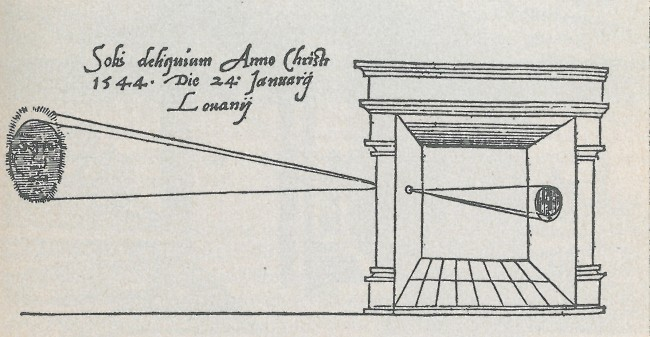
\includegraphics[width=0.79\textwidth]{camera-obscura.jpg}
	\caption{Camera obscura \cite{frisiusradio}.}
\end{figure}

\section{Pinhole Camera}
\begin{itemize}
	\item Pinhole size $=$ aperture
	\begin{itemize}
		\item too big $\Rightarrow$ blurring
		\item too small $\Rightarrow$ also blur, but because of diffraction\\ but then, \hlb{image is dark}
	\end{itemize}
	$\Rightarrow$ Use lenses: keep image sharp while \hlb{capture more light}
	\item The thin lens
	\item Focus \& Depth of Field:
	\begin{itemize}
		\item Large aperture: small depth of field\\
		(only object within the correct distance will be at focus, while background is blur)
		\item Small aperture: large depth of field, but need more light
	\end{itemize}
	\item The lens focus $f \gtrless$ field of view
	\begin{figure}[hbt!]
		\centering
		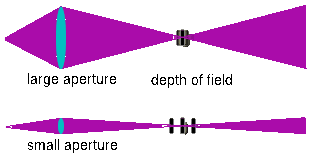
\includegraphics[width=0.57\textwidth]{depth-of-field.png}
		\caption{Varied depths of field depending on aperture size.}
	\end{figure}
	\begin{itemize}
		\item $f$ gets smaller $\Rightarrow$ wide-range image
		\item $f$ gets greater $\Rightarrow$ telescopic image
	\end{itemize}
\end{itemize}

\section{Digital image}
\begin{itemize}
	\item Discretize the image into a grid of pixels
	\item Quantize light intensities $\Rightarrow$ pixel values
	\item Resolution: \ac{no} pixels (most commonly understand)
\end{itemize}

\section{Color Sensing}
Referring to the process of assigning pixel values from color information of world objects.
\begin{itemize}
	\item Color image: RGB is just 1 of many color spaces, \eg, LUV, XYZ (\href{https://en.wikipedia.org/wiki/List_of_color_spaces_and_their_uses}{Wikipedia}).
	\item Grey-scale image
\end{itemize}

\subsection{Demosaicing}
Digital camera takes in light through a filter (Bayer or Xtrans) $\Rightarrow$ we get a gray-scale image (\figref{fig:demosaicing}). We need to apply demosaicing based on the filter's pattern to get the color image from the raw image. Sources: \href{https://www.youtube.com/watch?v=9cPxEFpg3Eg}{YouTube}, \href{https://en.wikipedia.org/wiki/Demosaicing}{Wikipedia}.
\begin{figure}[hbt!]
	\centering
	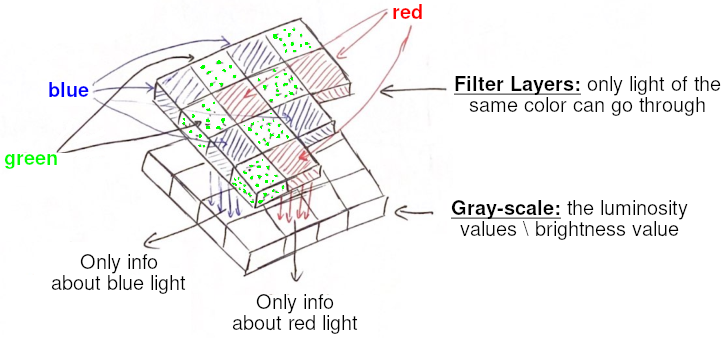
\includegraphics[width=\textwidth]{demosaicing.png}
	\caption{\Eg Bayer Filter. In the raw image , which lies below the filter layers, each pixel only has \ac{info} of only 1 among 3 light sources. Demosaicing uses the values of surrounding pixels to infer the brightness of other light sources.}
	\label{fig:demosaicing}
\end{figure}

\note Raw image has a \hlb{green cast}\\
Twice many green as red \& blue, because human eyes are twice as sensitive to the green part to other red or blue part.

	% !TeX spellcheck = en_US
\chapter{Image Processing}

\section{Linear Filters}
Types of noise:
\begin{itemize}
	\item Salt \& pepper noise
	\item Impulse noise
	\item Gaussian noise\\
	$noise = randn(size(img)) \times \sigma$\\
	$output = img + noise$
	\item \hlr{\underline{Basic assumption:}} \ac{iid}
\end{itemize}
Types of filter:
\begin{itemize}
	\item Correlation Filter: $\displaystyle G[i,j] = \frac{1}{(2k+1)^2} \sum_{u=-k}^{k} \sum_{v=-k}^{k} F[i+u, j+v] $\\
	different weights: $\displaystyle G[i,j] = \sum_{u=-k}^{k} \sum_{v=-k}^{k} H[u,v]F[i+u, j+v] \Rightarrow {\color{red} \boxed{G = H \otimes F}}$\\
	with $H[u,v]$ as non-uniform weights\\
	\hlb{Matlab:} \texttt{filter2, imfilter}
	\item Convolution: \tab $\displaystyle G[i,j] = \sum_{u=-k}^{k} \sum_{v=-k}^{k} H[u,v]F[i-u, j-v] \Rightarrow {\color{red} \boxed{G = H * F}}$\\
	\hlb{Matlab:} \texttt{conv2}\\
	\hlr{If $H[u,v] = H[-u,-v] \Rightarrow$ correlation $\equiv$ convolution}
	\item Averaging Filter: \hlr{Ringing Artifacts??}
	\item Gaussian Filter: $\displaystyle \frac{1}{\sqrt{2\pi}} \exp \left(-\frac{(x-\mu)^2}{2\sigma^2}\right)$\\
	\hlb{Rule of thumb:} set the filter width to $6\sigma$\\
	\hlr{More noise $\Rightarrow\;\; \uparrow \sigma \Rightarrow$ blurring effect}
\end{itemize}

\note
\begin{itemize}
	\item \hlr{$k$ is from the window size $(2k+1)\times(2k+1)$}
	\item \hlr{Efficient implementation:} if filter is separable $\Rightarrow$ apply 1D filter 2 times to have a 2D filter $\Rightarrow$ Reduce the computational cost from $\mathcal{O}(K^2)$ to $\mathcal{O}(2K)$, with $K$ as the kernel size
	\item When coding with \texttt{Python}, the origin of image plane is top left corner, $x$-axis goes left, $y$-axis goes downward (\figref{fig:image-coords})
	\begin{figure}[!htb]
		\centering
		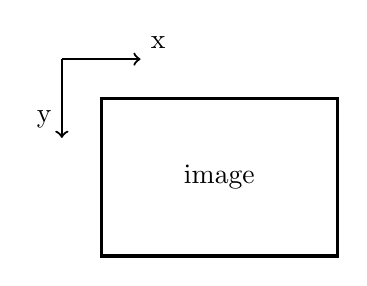
\begin{tikzpicture}			
			\draw[thick,->] (0,0) -- (1,0) node[anchor=south west] {x};
			\draw[thick,->] (0,0) -- (0,-1) node[anchor=south east] {y};
			\draw[very thick] (0.5,-0.5)  rectangle (3.5,-2.5) node[pos=.5]{image};
		\end{tikzpicture}
		\caption{Image coordinate system in \texttt{Python}}	
		\label{fig:image-coords}
	\end{figure}
	\item Boundary issues:
	\begin{align*}
		&\text{- Full: }  \tab \text{output size} = f+g && 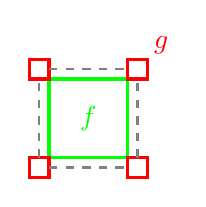
\begin{tikzpicture}[scale=0.5]\draw[green, very thick] (0,0) rectangle (2,2) node[pos=.5]{$f$};
			\draw[red, very thick] (2,2) rectangle (2.5,2.5) node[pos=1.7]{$g$};
			\draw[red, very thick] (0,0) rectangle (-.5,-.5);
			\draw[red, very thick] (2,0) rectangle (2.5,-.5);
			\draw[red, very thick] (0,2) rectangle (-.5,2.5);
			\draw[gray, thick, dashed] (-.25,0) -- (-.25,2);
			\draw[gray, thick, dashed] (0,-.25) -- (2,-.25);
			\draw[gray, thick, dashed] (2.25,0) -- (2.25,2);
			\draw[gray, thick, dashed] (0,2.25) -- (2,2.25);
		\end{tikzpicture}\\
		&\text{- Same:}  \tab \text{output size} = f   && 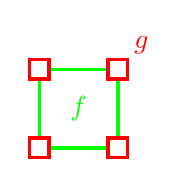
\begin{tikzpicture}[scale=0.5]\draw[green, very thick] (0,0) rectangle (2,2) node[pos=.5]{$f$};
			\draw[red, very thick, fill=white] (1.75,1.75) rectangle (2.25,2.25) node[pos=1.7]{$g$};
			\draw[red, very thick, fill=white] (1.75,-.25) rectangle (2.25,.25);
			\draw[red, very thick, fill=white] (-.25,-.25) rectangle (.25,.25);
			\draw[red, very thick, fill=white] (-.25,1.75) rectangle (.25,2.25);
		\end{tikzpicture}\\
		&\text{- Valid:} \tab \text{output size} = f-g && 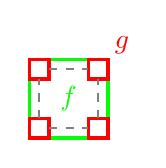
\begin{tikzpicture}[scale=0.5]\draw[green, very thick] (0,0) rectangle (2,2) node[pos=.5]{$f$};
			\draw[red, very thick] (1.5,1.5) rectangle (2,2) node[pos=1.7]{$g$};
			\draw[red, very thick] (0,0) rectangle (.5,.5);
			\draw[red, very thick] (2,0) rectangle (1.5,.5);
			\draw[red, very thick] (0,2) rectangle (.5,1.5);
			\draw[gray, thick, dashed] (.5,.25) -- (1.5,0.25);
			\draw[gray, thick, dashed] (.25,.5) -- (.25,1.5);
			\draw[gray, thick, dashed] (1.75,.5) -- (1.75,1.5);
			\draw[gray, thick, dashed] (.5,1.75) -- (1.5,1.75);
		\end{tikzpicture}
	\end{align*}
	\hlb{Pixel near boundary}:
	\begin{itemize}
		\item Clip filter (black) $\Rightarrow$ dark border
		\item Wrap around
		\item Copy edge $\Rightarrow$ Strong edge response
		\item Reflect across edge
	\end{itemize}
	\item Correlation \ac{vs} convolution:
	\begin{itemize}
		\item Both are linear shift invariant \ac{LSI}:\\
		\tab $h \circ (f_0 + f_1) = h \circ f_1 + h \circ f_0$
		\item Conv is better, it has additional nice properties
		\begin{itemize}
			\item commutative: $f*g = g*f$
			\item associative: $(f*g)*h = f*(g*h)$
			\item Fourier transform $f*g \multimap F.G$ and $f.h \multimap F*H$
		\end{itemize}
		\item With impulse image, Conv reproduces itself, while Corr reflects itself.
	\end{itemize}	
\end{itemize}

\section{Background}
\begin{itemize}
	\item Taking the Fourier Transform of a signal $\Rightarrow$ Frequency coefficients $\Rightarrow$ \hlb{Frequency Spectrum}\\
	\hlr{\underline{Duality:}} $\;$The \hlr{better} a function is \hlr{localized} in one domain\\
	\tab\tab the \hlr{worse} it is \hlr{localized} in the other domain.
	\item Effect of Convolution: $ f * g \multimap F \cdot G$\\
	taking convolution in one domain is equivalent to multiplication in the other domain\\
	A Guassian has compact support in both domains\\
	$\Rightarrow$ \hlb{convenient choice} for \hlr{low-pass filter}
	\item Sharpening filter - \hlr{high-pass filter}: emphasizes noise as well
\end{itemize}
\begin{figure}[!htb]
	\centering
	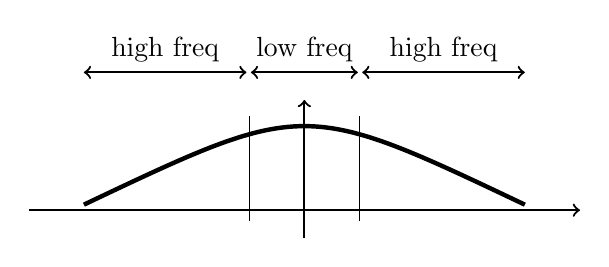
\begin{tikzpicture}[scale=0.7]
		\draw[thick,->] (-5,0) -- (5,0);
		\draw[thick,->] (0,-.5) -- (0,2);
		\draw[ultra thick] (-4,.1) .. controls (0,2) .. (4,.1);
		\draw[thin] (-1,-.2) -- (-1,1.7);
		\draw[thin] (1,-.2)  -- (1,1.7);
		\draw[thick,<->] (-4,2.5) -- (-1.05,2.5) node[pos=0.5, above=0.2]{high freq};
		\draw[thick,<->] (1.05,2.5) -- (4,2.5) node[pos=0.5, above=0.2]{high freq};
		\draw[thick,<->] (-0.97,2.5) -- (0.97,2.5) node[pos=0.5, above=0.2]{low freq};
	\end{tikzpicture}
	\caption{Frequency domain (Fourier).}
	\label{fig:freq-domain}
\end{figure}

\section{Non-Linear Filters}
\begin{itemize}
	\item Median filter: replace each pixel by the median of the neighbors.
	\begin{itemize}
		\item \hlr{remove spikes} (good for impulse, salt \& pepper noise)
		\item \hlr{edge preserving} (unlike mean filter)
	\end{itemize}
	\note If we increase the Median filter's filter size $\Rightarrow$ reduce structure and loose details
\end{itemize}

\section{Multi-Scale Representations}
Image pyramid: very \hlb{little overhead} (in terms of \hlb{computational cost}).

\hlb{Fourier Interpretation:} Discrete Sampling\\
Sampling in spatial domain is like \hlb{multiplying with a spike \ac{func}}.

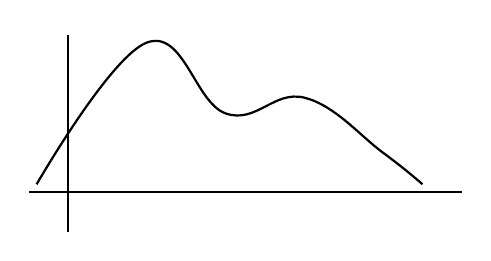
\begin{tikzpicture}
	\draw[thick] (-.5,0) -- (5,0);
	\draw[thick] (0,-.5) -- (0,2);
	\draw[thick] plot [smooth, tension=.7] coordinates {(-.4,.1) (1,1.9) (2,1) (3,1.2) (4, .5) (4.5,0.1)};
\end{tikzpicture}

$\Rightarrow$ Sampling in the frequency domain is like \hlb{convolving with a spike \ac{func}}.

\section{Filters as Templates}
Correlation filtering as Template Matching.

\section{Image Gradients}


\section{Edge Detection}


\section{Structure Extraction}

\todo{missing content}
	% !TeX spellcheck = en_US
\chapter{Segmentation}
\todo{}
	% !TeX spellcheck = en_US
\chapter{Object Detection}
\todo{}
	% !TeX spellcheck = en_US
\chapter{Local Feature}
\todo{}
	% !TeX spellcheck = en_US
\chapter{Deep Learning for CV}
\todo{}

\section{Loss Functions}
L1-L2 loss doesn't work well with different \ac{CV} problems \cite{wang2009mean}. This section proposes some alternatives

\subsection{SSIM}
\ac{SSIM} measures the similarity between two images. \cite{wang2004image}
\begin{itemize}
	\item The \ac{SSIM} index is calculated on various windows of an image.
	\item Formula: Given two windows $x, y \in \mathbb{R}^{N \times N}$ (check \href{https://en.wikipedia.org/wiki/Structural_similarity}{Wikipedia})
	\begin{align}
		\text{SSIM}(x,y) &= \frac{(2\mu_x \mu_y + c_1) (2\sigma_{xy} + c_2)}{(\mu_x^2 + \mu_y^2 + c_1) (\sigma_x^2 + \sigma_y^2 + c_2)}\\
		\text{SSIM}(x,y) &= luminance(x,y) \cdot contrast(x,y) \cdot structure(x,y)
	\end{align}
	\item It is used in super-resolution problem.
\end{itemize}

\subsection{Perceptual Loss}
\label{subsec:perceptual-loss}
\begin{itemize}
	\item Perceptual Loss, \ac{aka} content loss or VGG loss, is the loss between the feature maps of two images, after passing through a few pretrained \ac{CNN} layers (\figref{fig:vgg-loss}).
	\item This loss is used in super-resolution problem
\end{itemize}

\begin{figure}[hbt!]
	\centering
	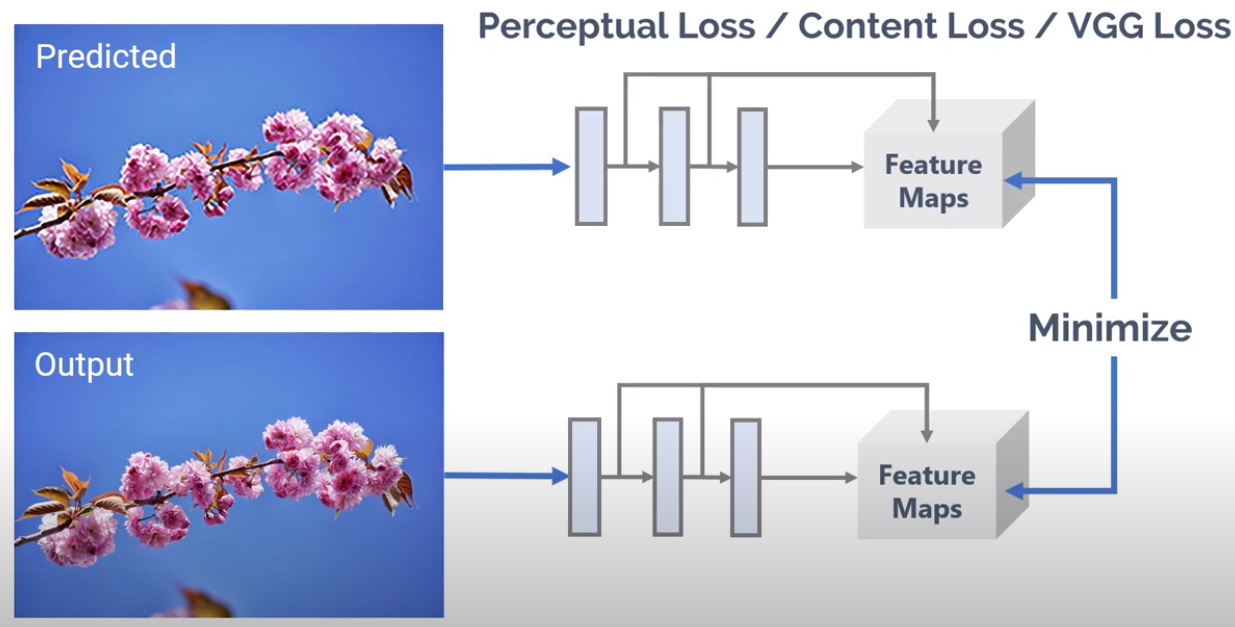
\includegraphics[width=0.7\textwidth]{vgg-loss.png}
	\caption{Perceptual loss is the loss between the feature maps, which are from passing images through a few frozen \ac{CNN} layers from VGG network.}
	\label{fig:vgg-loss}
\end{figure}

\subsection{FID}
In \ac{CV}, \ac{FID} is used to measure the distance between two distributions of two datasets, which are usually the original and the generated image datasets. \cite{heusel2017gans}
\begin{itemize}
	\item Pass the images through the pretrained Inception network, take the output right before the last layer.
	\item Calculate the mean and covariance matrices: $(\textbf{\textit{m}}, \textbf{\textit{C}})$ and $(\textbf{\textit{m}}_w, \textbf{\textit{C}}_w)$
	\begin{equation}
		d^2((\textbf{\textit{m}}, \textbf{\textit{C}}), (\textbf{\textit{m}}_w, \textbf{\textit{C}}_w)) = ||\textbf{\textit{m}} - \textit{\textbf{m}}_w||_2^2 + \text{Tr}(\textbf{\textit{C}} + \textbf{\textit{C}}_w - 2(\textbf{\textit{CC}}_w)^{1/2})
	\end{equation}
	\item The smaller the \ac{FID} value the better the generated images, obviously.
\end{itemize}

\subsection{PPL}
The high-level idea is such, when interpolation in the latent space may lead to non-linear changes in the image. 
\ac{PPL} is a metric to measure  the perceptually-based pairwise image distance. \cite{karras2019style}

\begin{align}
	l_{\mathcal{Z}} &= \mathbb{E} \left[ \frac{1}{\epsilon^2} d\left(G(\text{slerp}(\textbf{z}_1, \textbf{z}_2; t)), G(\text{slerp}(\textbf{z}_1, \textbf{z}_2; t + \epsilon))\right) \right] && \text{average in $\mathcal{Z}$ space}\\
	l_{\mathcal{W}} &= \mathbb{E} \left[ \frac{1}{\epsilon^2} d\left(g(\text{lerp}(f(\textbf{z}_1), f(\textbf{z}_2); t)), g(\text{lerp}(f(\textbf{z}_1), f(\textbf{z}_2); t + \epsilon))\right) \right] && \text{average in $\mathcal{W}$ space}
\end{align}

\begin{itemize}
	\item Latent vectors $\textbf{z}_1, \textbf{z}_2 \sim P(\textbf{z})$
	\item Interpolation functions: slerp and lerp.\\
	Basically, they also output a latent vector that lie on the interpolation path from $\textbf{z}_1$ to $\textbf{z}_2$
	\[\textbf{z}_t = \text{slerp}(\textbf{z}_1, \textbf{z}_2; t) \quad \text{with} \ t \sim U(0,1)\]
	\item $G$ is the generator, $g$ is the synthesis network, $f$ is the mapping network, thus $G = g \circ f$ and $image = G(\textbf{z})$ (\figref{fig:stylegan-generator})
	\item $d$ evaluates the perceptual loss given two generated images (\subsecref{subsec:perceptual-loss})
\end{itemize}

\section{Image-to-Image Translation}
Image-to-image translation is a class of \ac{CV} problems where the goal is to learn the mapping between an input image and an output image. Recent approaches utilize \ac{GAN}. It has various applications \cite{isola2017image, zhu2017unpaired}, \eg:
\begin{itemize}
	\item Domain adaptation
	\item Semantic label $\leftrightarrow$ photo
	\item Map $\leftrightarrow$ aerial photo
	\item Edges $\rightarrow$ photo
	\item BW $\rightarrow$ color photos
	\item Day $\rightarrow$ night
	\item Photo with missing pixels $\rightarrow$ inpainted photo (recovering)
\end{itemize}

\subsection{pix2pix}
\texttt{pix2pix} uses \ac{CGAN} idea with U-Net architecture \cite{isola2017image}.
\begin{figure}[hbt!]
	\centering
	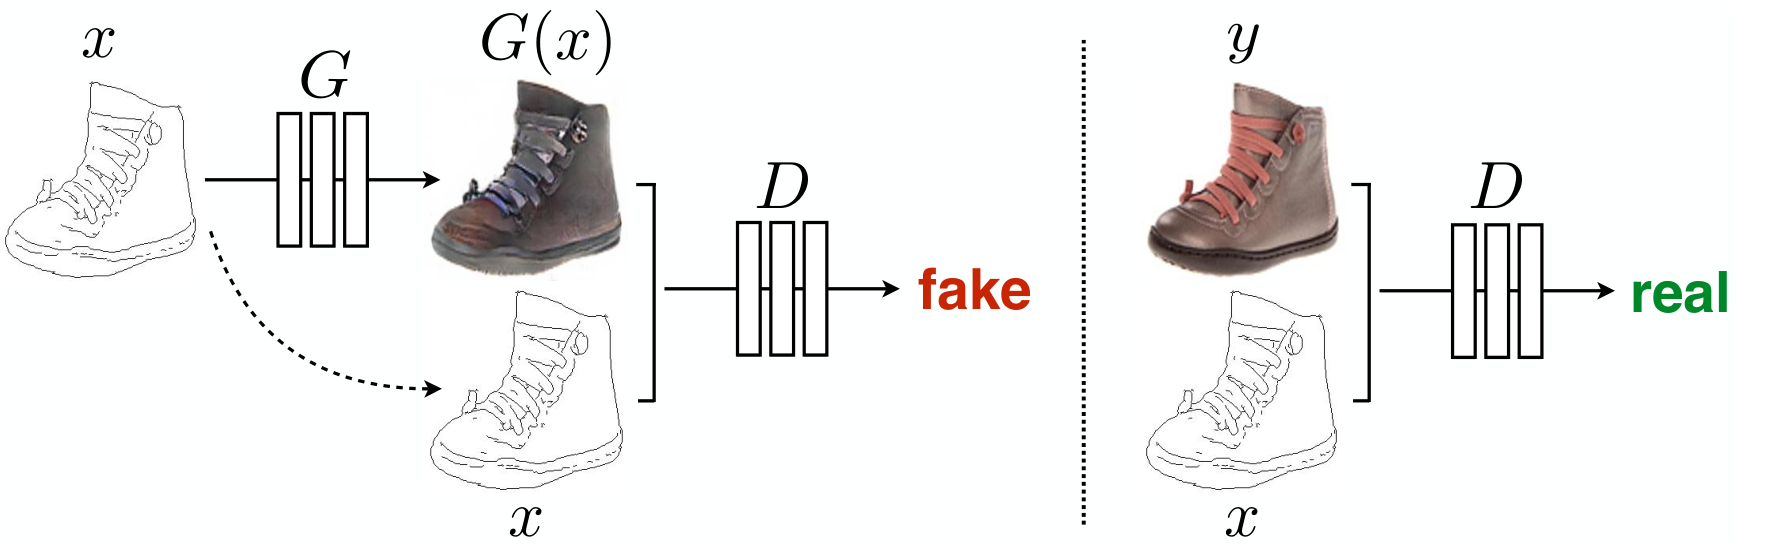
\includegraphics[width=0.9\textwidth]{pix2pix.png}
	\caption{Training a \ac{CGAN} to map edges $\rightarrow$ photo. Both the discriminator and generator are conditioned on the input $x$. \cite{isola2017image}}
\end{figure}

The loss function of \texttt{pix2pix} combines \ac{CGAN} objective with L1 distance with ground-truth images. L1 distance is prefer over L2 because L1 encourages less blurring effect.
\begin{align}
	\mathcal{L}_{GAN}(G,D) &= \mathbb{E}_y [\log D(y)] + \mathbb{E}_z [\log (1-D(G(z)))]\\
	\mathcal{L}_{CGAN}(G,D) &= \mathbb{E}_{x,y} [\log D(x,y)] + \mathbb{E}_{x,z} [\log (1-D(x,G(x,z)))]\\
	\mathcal{L}_{L1}(G) &= \mathbb{E}_{x,y,z} \big[ ||y-G(x,z)||_1 \big]\\
	G* &= \arg \underset{G}{\min} \underset{D}{\max} \mathcal{L}_{CGAN}(G,D) + \lambda \mathcal{L}_{L1}(G)
\end{align}

\note In implementation, the noise $z$ is accounted as DropOut percentage.

\subsection{CycleGAN}
Cycle\ac{GAN} addresses the problem when there is no \hlb{available paired training data}. By considering cycle consistency losses, it limits the mapping functions. \cite{zhu2017unpaired}
\begin{align}
	&G: X \rightarrow Y &&-\text{mapping from domain $X$ to domain $Y$}\\
	&F: Y \rightarrow X &&-\text{mapping from domain $Y$ to domain $X$}\\
	&F(G(x)) \approx x &&-\text{forward cycle consistency}\\
	&G(F(y)) \approx y &&-\text{backward cycle consistency}
\end{align}
\begin{align}
	\mathcal{L}_{GAN_1} (G, D_Y, X, Y) &= \mathbb{E}_{y \sim p_{data}(y)}[\log D_Y(y)] + \mathbb{E}_{x \sim p_{data}(x)} [\log (1 - D_Y(G(x)))]\\
	\mathcal{L}_{GAN_2} (F, D_X, X, Y) &= \mathbb{E}_{x \sim p_{data}(x)}[\log D_X(x)] + \mathbb{E}_{y \sim p_{data}(y)} [\log (1 - D_X(F(y)))]\\
	\mathcal{L}_{cyc}(G,F) &= \mathbb{E}_{x \sim p_{data}(x)}\big[||F(G(x))-x||_1 \big] + \mathbb{E}_{y \sim p_{data}(y)} \big[||G(F(y))-y||_1\big]\\
	\mathcal{L}(G, F, D_X, D_Y) &= \mathcal{L}_{GAN_1} (G, D_Y, X, Y) + \mathcal{L}_{GAN_2} (F, D_X, X, Y) + \lambda \mathcal{L}_{cyc}(G,F)\\
	G^*, F^* &= \arg\underset{G, F}{\min}\underset{D_X, D_Y}{\max} \mathcal{L}(G, F, D_X, D_Y)
\end{align}
\begin{figure}[hbt!]
	\centering
	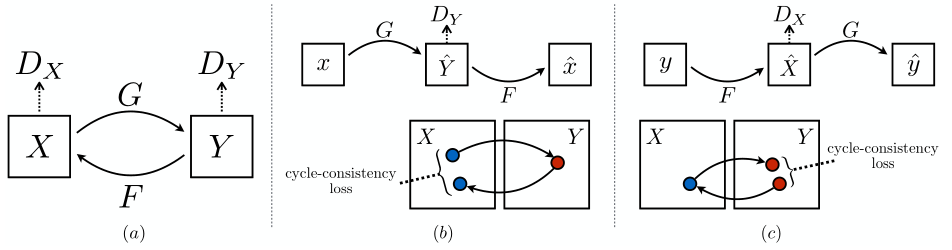
\includegraphics[width=\textwidth]{cyclegan.png}
	\caption{Cycle\ac{GAN} structure with 4 networks. \cite{zhu2017unpaired}}
\end{figure}

\note
\begin{itemize}
	\item The authors mention that experiment the cycle consistency loss as adversarial loss leads to no improved performance.
	\item Cycle\ac{GAN}'s results are not significantly better than pix2pix's.
	\item Perform well on tasks relating color transformation (\eg style transfer: picture $\leftrightarrow$ paintings, horse $\leftrightarrow$ zebra, winter $\leftrightarrow$ summer), but not so good with \hlb{geometric changes} (dog $\leftrightarrow$ cat).
\end{itemize}

\section{Neural Style Transfer}
Style transfer is similar to image-to-image translation, but doesn't require a dataset from each style. It instead runs an iterative optimization procedure on two given images.

\subsection{Artistic Style Transfer}
The first work is by \citeaus{gatys2015neural}. The authors manage to separate image content and image style. Given a \ac{CNN}, at the $l^{th}$ layer, there is $N_l$ distinct filters, thus, leads to $N_l$ feature maps of size $M_l$.
\begin{itemize}
	\item The image content is represented in matrix $F^l \in \mathcal{R}^{N_l \times M_l}$, which is the concatenation of these feature maps. $F^l_{ij}$ is the activation of the $i^{th}$ filter at position $j$ in $l^{th}$ layer. The authors prove this by trying to reconstruct the image from these feature maps.
	\begin{align}
		&\vec{p} &&-\text{original image}\\
		&\vec{x} &&-\text{generated image}\\
		&F^l_{ij} &&-\text{the original image's content }\\
		&P^l_{ij} &&-\text{the generated image's content}\\
		&\mathcal{L}_{content}(\vec{p}, \vec{x}, l) = \frac{1}{2} \sum_{i,j} \left( F^l_{ij} - P^l_{ij} \right) ^2 &&-\text{the content loss}
	\end{align}
	\item The image style is represented in the Gram matrix $G^l \in \mathcal{R}^{N_l \times N_l}$, where $G_{ij}^l$ is the correlation between feature map in the $l^{th}$ layer:
	\begin{equation}
		G_{ij}^l = \sum_k F_{ik}^l F_{jk}^l
	\end{equation}
	\begin{align}
		&\vec{a} &&-\text{artwork}\\
		&\vec{x} &&-\text{generated image}\\
		&A^l &&-\text{the artwork's style representation}\\
		&G^l &&-\text{the generated image's style representation}\\
		&E_l = \frac{1}{4 N^2_l M^2_l} \sum_{i,j} \left( G_{ij}^l - A_{ij}^l \right)^2 &&-\text{style representation loss at $l^{th}$ layer}	\\
		&\mathcal{L}_{style}(\vec{a}, \vec{x}) = \sum_{l=0}^L w_l E_l &&-\text{the style loss}
	\end{align}
\end{itemize}
\begin{align}
	&\mathcal{L}_{total}(\vec{p}, \vec{a}, \vec{x}) =  \alpha \mathcal{L}_{content}(\vec{p}, \vec{x})+ \beta \mathcal{L}_{style}(\vec{a}, \vec{x}) &&-\text{total loss}
\end{align}

The algorithm applies gradient descent to minimize the above loss with $\vec{x}$ as a white noise image in the beginning.

\subsection{Artistic Style Transfer for Videos}
Applying the above approach to video leads to terribly inconsistent results. \citeaus{ruder2016artistic} improve by adding additional improvements:
\begin{itemize}
	\item Short-term consistency by initialization: Estimate the optical flow between image $p^{(i)}$ and $p^{(i+1)}$. The generated image $x^{(i+1)}$ will not be initialized with a white noise image, but a warped image from the previous one: $x'^{(i+1)} = \omega_i^{i+1} (x^{(i)})$. Here $\omega_i^{i+1}$ denotes the warping function using the estimated optical flow.
	\item Temporal consistency loss
	\item Long-term consistency
	\item Multi-pass algorithm
\end{itemize}

\subsection{Fast Artistic Style Transfer}
The above style transfer approaches require an iterative optimization process for each pair of images. \citeaus{johnson2016perceptual} propose a training pipeline to simplify this procedure. By learning a network that minimize the same loss, the output now requires only one single run.
\begin{figure}[hbt!]
	\centering
	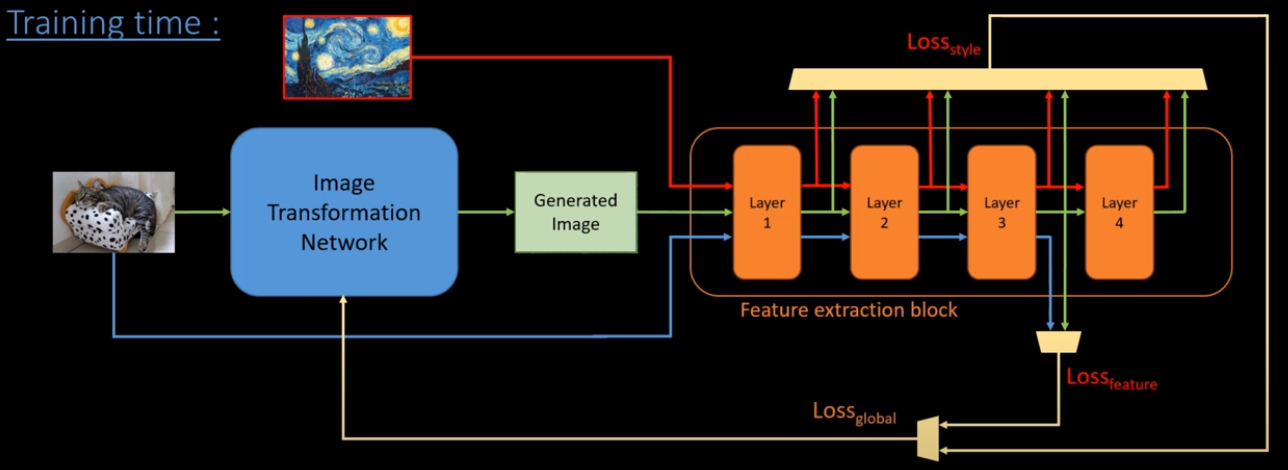
\includegraphics[width=\textwidth]{fast-artistic-style-transfer.png}
	\caption{Training pipeline (\href{https://youtu.be/VQEMptfWpLk}{src}) \cite{johnson2016perceptual}}
\end{figure}

\[\begin{matrix*}[l]
	\color{Green} + \text{Running in real-time}\\
	\color{red} - \text{Loss some temporal consistency when applying to videos}\\
	\color{red} - \text{One single style for a network}
\end{matrix*}\]

\subsection{Arbitrary Style-Transfer in Real-time}
\citeaus{huang2017arbitrary} improves prior methods::
\begin{itemize}
	\item Using \ac{AdaIN}
	\item Pros: $\begin{matrix*}[l]
		\color{Green} + \text{Running in real-time}\\
		\color{Green} + \text{A single network capable of transfer multiple arbitrary styles}
	\end{matrix*}$
\end{itemize}

Check their \href{https://youtu.be/IIRxJvW6bE4}{CVF presentation video}.

\section{Super Resolution}
Super Resolution is a \ac{CV} problem, in which we want to upscale a lower resolution image to a higher resolution one.
\begin{itemize}
	\item \href{https://youtu.be/KULkSwLk62I}{Youtube: How Super Resolution Works}
	\item Naive approach: nearest neighbor would simply spread the pixels out, then fill in the gap by copying values.
	\item Taking average, median would lead to better result, which is what bilinear and bicubic interpolation do.
\end{itemize}

\subsection{SRCNN}
\citeausm{dong2015image}'s model is a \ac{CNN} that (\figref{fig:SRCNN})
\begin{itemize}
	\item takes in a lower resolution image and output a higher resolution image
	\item the loss is simply squared error between the output with ground truth image
\end{itemize}

\begin{figure}[hbt!]
	\centering
	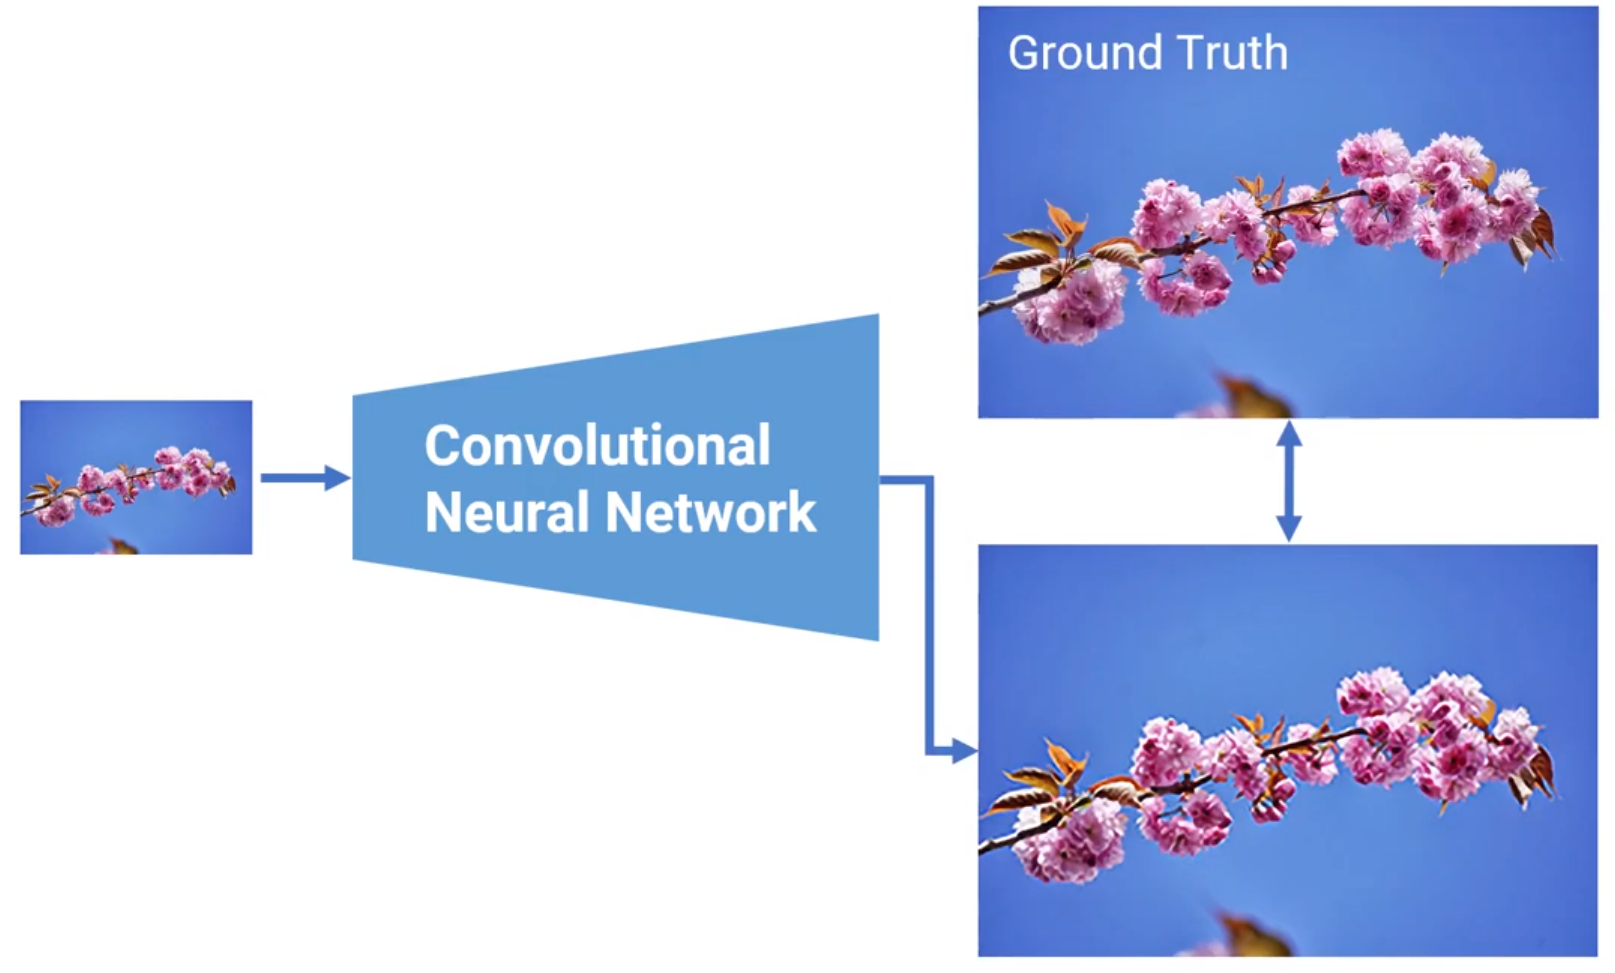
\includegraphics[width=0.7\textwidth]{SRCNN.png}
	\caption{\ac{SRCNN} training \cite{dong2015image}}
	\label{fig:SRCNN}
\end{figure}

\subsection{SRGAN}
\citeausm{ledig2017photo} use \ac{GAN}'s framework (\figref{fig:SRGAN}). The authors use VGG-based loss function

\begin{figure}[hbt!]
	\centering
	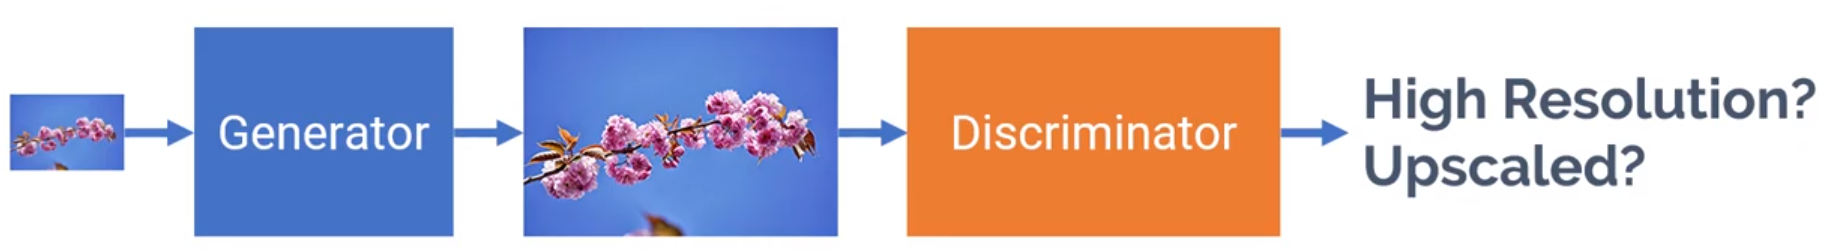
\includegraphics[width=\textwidth]{SRGAN.png}
	\caption{\ac{SRGAN} training \cite{ledig2017photo}}
	\label{fig:SRGAN}
\end{figure}

\subsection{ESRGAN}
\ac{ESRGAN} \cite{wang2018esrgan}
\begin{itemize}
	\item Remove \ac{BatchNorm}
	\item More layers and connections: residual scaling
	\item Modify the VGG loss: compare the feature maps before activation layers.
	\item Relativistic discriminator
\end{itemize}

\subsection{Further Improvements}
\begin{itemize}
	\item Network interpolation \cite{wang2018esrgan, wang2019deep}
	\item Contextual bilateral loss \cite{zhang2019zoom}
	\item Real-\ac{ESRGAN} \cite{wang2021realesrgan}
\end{itemize}

\subsection{Codes}
\begin{itemize}
	\item \href{https://github.com/xinntao/ESRGAN}{\ac{ESRGAN}} \cite{wang2018esrgan}
	\item \href{https://github.com/xinntao/Real-ESRGAN}{Real-\ac{ESRGAN}} \cite{wang2021realesrgan}
\end{itemize}

\section{StyleGAN}
\subsection{Initial Work}
\begin{itemize}
	\item Watch \href{https://youtu.be/kSLJriaOumA}{Tero Karras FI Youtube video}
	\item StyleGAN is image generation with style control. \cite{karras2019style}
	\item Key points on StyleGAN.v1's structure (\figref{fig:stylegan-generator}):
	\begin{itemize}
		\item Add mapping and styles via mapping network $f$ and \ac{AdaIN}
		\item Replace traditional input with a learnable constant \texttt{$4 \times 4 \times 512$}
		\item Add noise inputs at different levels: coarse ($4^2-32^2$) to fine layers ($64^2-1024^2$) with different scaling $B$
		\item Mixing regularization: use different style inputs from different latent vectors at different levels
	\end{itemize}
\end{itemize}

\subsection{Slider stuff}
With some additional steps, one could create a slider to gradually change different attributes, \eg gender, hair styles (\href{https://youtu.be/dCKbRCUyop8}{Arxiv Insights}).

\subsection{Truncation Trick}
Drawing latent vectors from a truncated sampling space tends to improve average image quality, with some loss in variation:
\begin{itemize}
	\item Compute center of mass of $\mathcal{W}$: $\bar{\textbf{w}} = \mathbb{E}_{\textbf{z} \sim P(\textbf{z})}[f(\textbf{z})]$
	\item Given a vector $\textbf{w}$, scale it: $\textbf{w}' = \bar{\textbf{w}} + \psi(\textbf{w} - \bar{\textbf{w}})$, where $|\psi| < 1$
	\item Varying $\psi$ value also gives us the nice interpolation effect (\figref{fig:stylegan-truncation})
	\begin{figure}[hbt!]
		\centering
		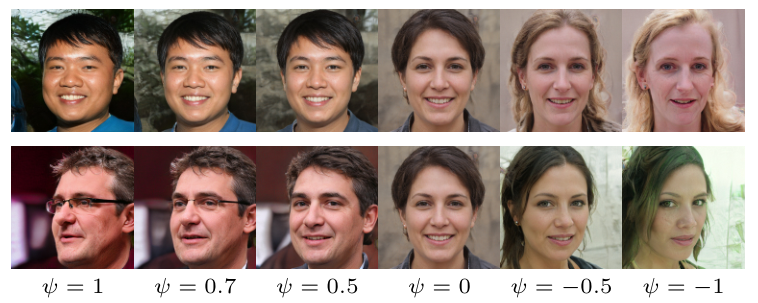
\includegraphics[width=0.7\textwidth]{stylegan-truncation.png}
		\caption{Effect of truncation trick}
		\label{fig:stylegan-truncation}
	\end{figure}
\end{itemize}

\subsection{Improvements}
Improvements to StyleGAN.v1 to handle droplet and phase artifacts:
\begin{itemize}
	\item \href{https://youtu.be/c-NJtV9Jvp0}{StyleGANv2} \cite{karras2020analyzing}
	\begin{itemize}
		\item Replacing \ac{AdaIN} with \ac{CNN} weight demodulation and moving addition of noise outside of style area (\figref{fig:stylegan-weight-demodulation})
		\begin{align}
			w'_{ijk} &= s_i \cdot w_{ijk}\\
			w''_{ijk} &= \frac{w'_{ijk}}{\sqrt{\sum_{i,k} {w'_{ijk}}^2 + \epsilon}}
		\end{align}
		\begin{figure}[hbt!]
			\centering
			\begin{subfigure}[b]{0.55\textwidth}
				\centering
				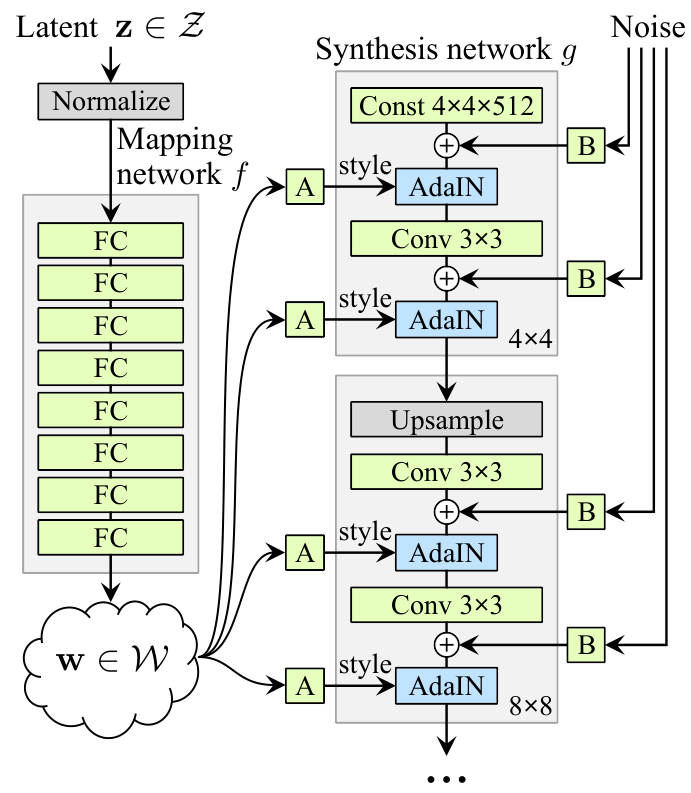
\includegraphics[width=\textwidth]{stylegan-generator.png}
				\caption{StyleGANv1's structure \cite{karras2019style}.}
				\label{fig:stylegan-generator}
			\end{subfigure}
			\hfill
			\begin{subfigure}[b]{0.4\textwidth}
				\centering
				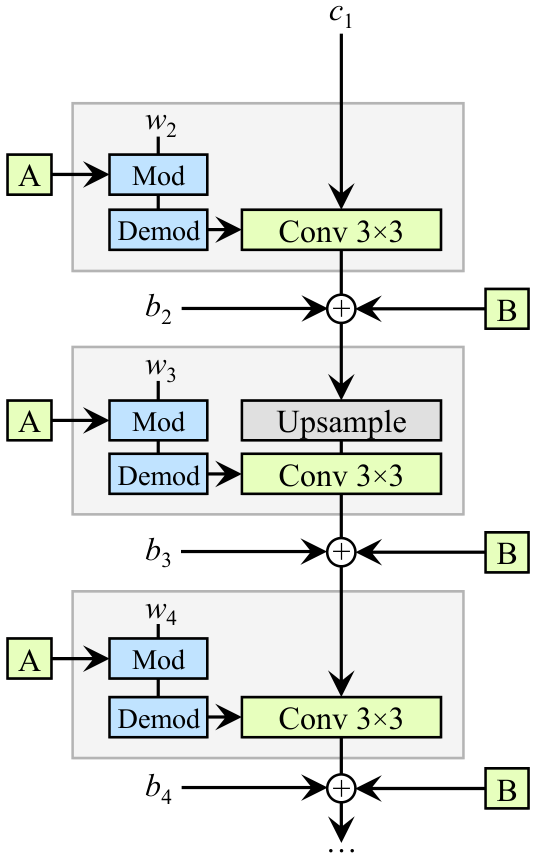
\includegraphics[width=\textwidth]{stylegan-weight-demodulation.png}
				\caption{Weight demodulation \cite{karras2020analyzing}.}
				\label{fig:stylegan-weight-demodulation}
			\end{subfigure}
			\caption{StyleGAN architectures.}
			\label{fig:stylegan}
		\end{figure}
		\item Lazy regularizer with \ac{PPL}
		\item Replacing progressive growing with skip connections and residual modules.
		\item Finally, it trains faster
	\end{itemize}
	\item StyleGAN3 suggests even more changes to deal with sticking texture artifacts (check \href{https://youtu.be/j1ZY7LInN9g}{bycloud} and \href{https://youtu.be/_euFoyLEyqU}{Andrew Melnik} videos) \cite{karras2021alias}
\end{itemize}

\section{Code Examples}
\begin{itemize}
	\item \href{https://www.tensorflow.org/tutorials/generative/pix2pix}{\texttt{Tensorflow}'s tutorial: pix2pix}
	\item \href{https://www.tensorflow.org/tutorials/generative/cyclegan}{\texttt{Tensorflow}'s tutorial: CycleGAN}
	\item \href{https://github.com/manuelruder/artistic-videos}{\texttt{Github} source code: Artistic Style Transfer for Videos}
	\item \href{https://www.tensorflow.org/tutorials/generative/style_transfer}{\texttt{Tensorflow}'s tutorial: Neural style transfer}
	\item \href{https://www.tensorflow.org/hub/tutorials/tf2_arbitrary_image_stylization}{\texttt{Tensorflow}'s tutorial: Fast Style Transfer}
\end{itemize}

	% !TeX spellcheck = en_US
\chapter{3D Computer Vision}
\label{cha:3D-cv}

\section{Introduction}
\label{sec:3D-cv-intro}
3D Computer Vision gives a representation that is closer of things that we interact in our lives. Thus, it will empower various novel applications in:
\begin{itemize}
	\item Autonomous Driving
	\item Robotics
	\item Remote Sensing
	\item Medical Treatment
	\item Design Industry
	\item Augmented Reality
\end{itemize}

\todo{} Learning resources: \href{https://??}{??}.

3D computer vision problems includes:
\begin{itemize}
	\item Depth extraction
	\item 3D Reconstruction
	\item Object Classification
	\item Object Detection
	\item Object Segmentation
	\item ??
\end{itemize}

Challenges of 3D computer vision:
\begin{itemize}
	\item something here
\end{itemize}

\section{Depth Extraction}
\hlb{The goal:} extract the depth, as the 3rd dimension for a 2D image.\\
The depth map is a simple grey image with values in range $[0, 255]$, $0$ for point afar and $255$ for points in near distances.
\begin{figure}[hbt!]
	\centering
	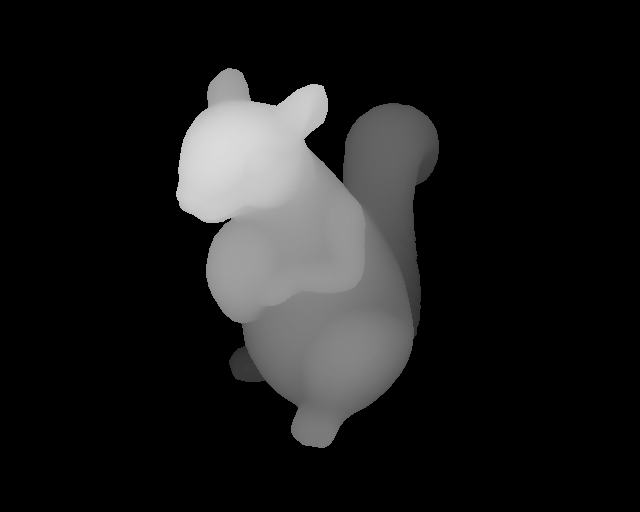
\includegraphics[width=0.57\textwidth]{depth-map.png}
	\caption{Example of a depth map \cite{tjaden2018}.}
\end{figure}

\section{3D Shape representation}
There are explicit representations and implicit representations, where parametric functions are used to differentiate a specific point is inside or outside the shape, or the distance to the shape surface. Typically, the parametric functions are in form of neural networks
\subsection{Voxel Grid}
\subsection{Point Cloud}
\subsection{Mesh}

\subsection{Occupancy}

\section{Classic 3D Reconstruction}
Geometric vision:
\begin{itemize}
	\item Visual Cues (Details)
	\begin{itemize}
		\item Shading
		\item Texture
		\item Focus
		\item Perspective
		\item Motion		
	\end{itemize}
	\item Stereo vision: process of extracting 3D information from multiple 2D views of a scene
\end{itemize}

\subsection{Epipolar Geometry}
Epipolar geometry is the geometry of stereo vision. The \hlr{basic principle} of epipolar geometry is \hlr{triangulation} of points.
\begin{figure}[hbt!]
	\centering
	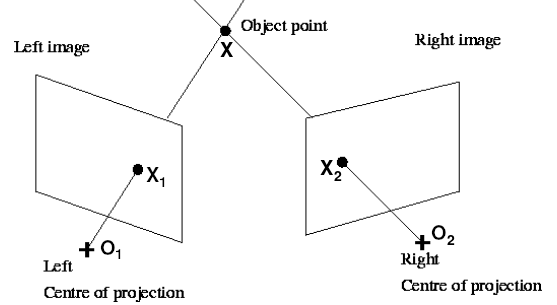
\includegraphics[width=0.57\textwidth]{triangulation.png}
	\caption{Example of triangulation (\href{https://homepages.inf.ed.ac.uk/rbf/CVonline/LOCAL_COPIES/OWENS/LECT10/node3.html}{src}). The lines connecting the camera poses with the correspondent points must intersect at the real object world space.}
	\label{fig:triangulation}
\end{figure}
In \figref{fig:triangulation}, $O_1$ and $O_2$ are the camera poses, $X_1$ and $X_2$ are the correspondent points on each image planes, and $X$ is the real object point in world space.

\todo{}

\subsection{Stereo Image Rectification}
Re-project image planes on to a common plane, which is parallel to the baseline\\
$\Rightarrow$ Scan lines are epipolar lines.

\todo{Add images}

\subsection{Correspondence Search}
Correspondence search simple means matching a point with another point in a different image.
\begin{table}[hbt!]
	\begin{tabularx}
		{\textwidth}{>{\setlength\hsize{\hsize}\setlength\linewidth{\hsize}}X|>{\setlength\hsize{\hsize}\setlength\linewidth{\hsize}}X}
		Dense Correspondence Search & Sparse Correspondence Search \\
		\hline
		\begin{itemize}
			\item For \hlr{each pixel}, find correspondence
			\item Easy when epipolar lines are scan lines (apply \hlr{rectification})
		\end{itemize} &
		\begin{itemize}
			\item Only for a set of detected feature
			\item Use feature description (Harris, SIFT??)
		\end{itemize}\\
		\multicolumn{2}{c}{------- \underline{Pros} -------}\\
		\begin{itemize}
			\item \hlr{Simple} process
			\item \hlr{More depth} $\Rightarrow$ useful for surface reconstruction
		\end{itemize} &
		\begin{itemize}
			\item \hlr{Efficiency}
			\item Can have more reliable matches
			\item Less sensitive to illumination $\Rightarrow$ \hlr{robust}
		\end{itemize}\\
		\multicolumn{2}{c}{------- \underline{Cons} -------}\\
		Problem with:
		\begin{itemize}
			\item \hlr{texture-less regions}
			\item different \hlr{viewpoints}
		\end{itemize} &
		\begin{itemize}
			\item Have to know enough to pick good features
			\item \hlr{Sparse} information
		\end{itemize}
	\end{tabularx}
\end{table}

\note \hlr{In practice, use both}.

\subsection{Stereo Reconstruction}
Main steps:
\begin{itemize}
	\item Calibrate cameras
	\item Rectify images
	\item Compute disparity
	\item Estimate depth
\end{itemize}
\hlr{This is just the \underline{ideal case}.}
\begin{itemize}
	\item What if, how can we get extrinsic \ac{info} from calibration?
	\item What to do when triangulation failed?
\end{itemize}

\subsection{Camera Calibration}
\subsection{Eight Point Algorithm}

\section{Deep Learning for 3D CV}


	% !TeX spellcheck = en_US
\chapter{Single Object Tracking}
\todo{}
	% !TeX spellcheck = en_US
\chapter{Bayesian Filtering}
\todo{}
	% !TeX spellcheck = en_US
\chapter{Multi Object Tracking}
\todo{}
	% !TeX spellcheck = en_US
\chapter{Visual Odometry}
\todo{}
	% !TeX spellcheck = en_US
\chapter{SLAM}
\todo{}
	% !TeX spellcheck = en_US
\chapter{Deep Learning for Video Analysis}
\todo{}
	\include{Contents/formulas.tex}
	% !TeX spellcheck = en_US
\chapter{Research Proposal}

There are levels of visual understanding
\begin{enumerate}
	{\item \color{Green} Object detection/classification}
	\item Detection of the state of an objects
	\item Detection of the relationships/interactions/compositions of objects
	\item Reasoning
\end{enumerate}

\section{Transfer Learning}

\section{Meta Learning}
	
	\backmatter
	\pagenumbering{Roman}
	\printbibliography[heading=bibintoc]
	\appendix
\end{document}